\begin{figure}[h]
    \centering
    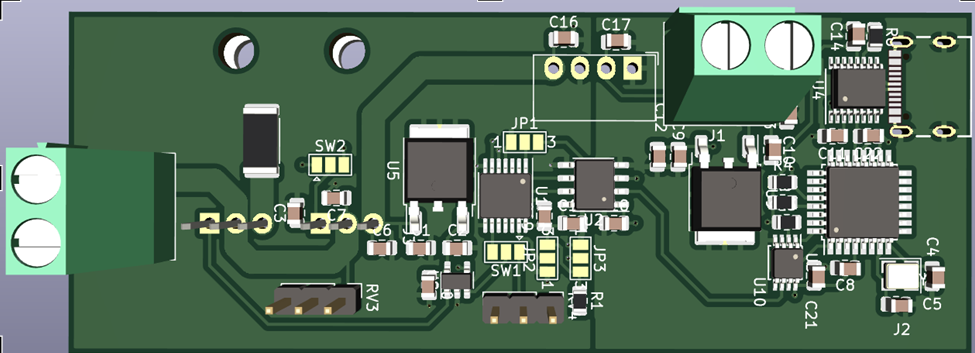
\includegraphics[scale=0.45]{pcb_1st_iteration.png}
    \caption{PCB layout of the 1st iteration of the emulator.}
    \label{fig:1st_pcb}
\end{figure}

A 3D model of the PCB is visible in Fig. \ref{fig:1st_pcb}.
The Fontys laser printer laboratory was used for the production 
of the first batch of PCBs, however, the via pressing equipment in the 
laboratory was incomplete, resulting in a fauty connections. 
This deemed the first PCB unusable, therefore the focus was 
immediately shifted to the second iteration, where the PCB 
would be ordered and made externally.
